\documentclass[a4paper,12pt,twoside,spanish]{book}
% Inicialización del documento

% Paquetes
\usepackage [spanish]{babel}
\usepackage[utf8]{inputenc}
\selectlanguage{spanish}
\usepackage[dvips]{graphicx}
\usepackage[colorlinks=true,linkcolor=black]{hyperref}
\usepackage{amsmath}
\usepackage{amsfonts}
\usepackage{mathptmx} % Times New Roman en LaTeX
\usepackage{amssymb}
\usepackage{anysize}
\usepackage{latexsym}
\usepackage{epsfig}
\usepackage{fancyhdr}
\usepackage{float}
\usepackage{colortbl}
\usepackage{color}
\usepackage{wrapfig}
\usepackage{subfigure}
\usepackage{epstopdf}
\usepackage{booktabs}
\usepackage[T1]{fontenc}
\usepackage[outermargin=-2.5cm,]{fullwidth}
\usepackage{boxedminipage}
\usepackage{shadow}
\usepackage{lscape}
\usepackage{titlesec}
\usepackage{curves}
\usepackage{rotating}
\usepackage{calc}
\usepackage{url}
\usepackage{babelbib}
\usepackage{hyperref}
\hypersetup{
   citecolor=black
}
\usepackage[justification=centering]{caption}
\usepackage{setspace}
\usepackage{nomencl}
\makenomenclature
\usepackage[nottoc]{tocbibind} % Para que aparezcan la tabla de figuras y cuadros en el índice
\renewcommand{\nomname}{Lista de acrónimos y abreviaturas}


\usepackage{listings}
\usepackage{xcolor}

\definecolor{codegreen}{rgb}{0,0.6,0}
\definecolor{codegray}{rgb}{0.5,0.5,0.5}
\definecolor{codepurple}{rgb}{0.58,0,0.82}
\definecolor{backcolour}{rgb}{0.95,0.95,0.92}

\lstdefinestyle{mystyle}{
	backgroundcolor=\color{backcolour},   
	commentstyle=\color{codegreen},
	keywordstyle=\color{magenta},
	numberstyle=\tiny\color{codegray},
	stringstyle=\color{codepurple},
	basicstyle=\ttfamily\footnotesize,
	breakatwhitespace=false,         
	breaklines=true,                 
	captionpos=b,                    
	keepspaces=true,                 
	numbers=left,                    
	numbersep=5pt,                  
	showspaces=false,                
	showstringspaces=false,
	showtabs=false,                  
	tabsize=2
}
\lstset{style=mystyle}

% Paquetes

% Formato de las páginas
\onehalfspace 
\raggedbottom
\pagestyle{fancy} 
\addtolength{\headwidth}{\marginparsep}
\setlength{\headheight}{25pt}
\setlength{\oddsidemargin}{0cm}
\setlength{\evensidemargin}{0cm}
\marginsize{2.5cm}{2.5cm}{2.5cm}{2.5cm}
\fancyhf{}
\fancyhead[LE,RO]{\bfseries \thepage} 
\fancyhead[LO]{\sffamily\scshape\footnotesize\rightmark} 
\fancyhead[RE]{\sffamily\scshape\footnotesize\leftmark} 
\addtolength{\parskip}{5pt}
% Formato de las páginas

\begin{document}
\chapter{Análisis script meshAP.py}
\section{Configuración del script meshAP.py}

Este fichero contiene la configuración de una red mesh simple que cuenta con dos access points y dos estaciones base. Dicha configuración corresponde a la de una red SDN en la que los access points funcionan como switches típicos de este tipo de redes.\par

El contenido del script meshAP.py es el siguiente: \par

\begin{lstlisting}
#!/usr/bin/python

"""
This example shows on how to create wireless link between two APs 
with mesh
The wireless mesh network is based on IEEE 802.11s
"""

from mininet.log import setLogLevel, info
from mn_wifi.link import wmediumd, mesh
from mn_wifi.cli import CLI
from mn_wifi.net import Mininet_wifi
from mn_wifi.wmediumdConnector import interference


def topology():
"Create a network."
net = Mininet_wifi(link=wmediumd, wmediumd_mode=interference)

info("*** Creating nodes\n")
sta1 = net.addStation('sta1', mac='00:00:00:00:00:11', 
	position='1,1,0')
sta2 = net.addStation('sta2', mac='00:00:00:00:00:12', 
	position='31,11,0')
ap1 = net.addAccessPoint('ap1', wlans=2, ssid='ssid1', 
	position='10,10,0')
ap2 = net.addAccessPoint('ap2', wlans=2, ssid='ssid2', 
	position='30,10,0')
c0 = net.addController('c0')

info("*** Configuring wifi nodes\n")
net.configureWifiNodes()

info("*** Associating Stations\n")
net.addLink(sta1, ap1)
net.addLink(sta2, ap2)
net.addLink(ap1, intf='ap1-wlan2', cls=mesh, ssid='mesh-ssid', 
	channel=5)
net.addLink(ap2, intf='ap2-wlan2', cls=mesh, ssid='mesh-ssid', 
	channel=5)

info("*** Starting network\n")
net.build()
c0.start()
ap1.start([c0])
ap2.start([c0])

info("*** Running CLI\n")
CLI(net)

info("*** Stopping network\n")
net.stop()


if __name__ == '__main__':
setLogLevel('info')
topology()
\end{lstlisting}

Se trata de una red mesh de medio inalámbrico \
($link=wmedium$) con interferencias ($wmedium\_mode=interference$). El simulador se encarga de calcular el nivel de interferencia en base a la distancia existente entre un nodo y sus nodos adyacentes. También se desprende del script que la red presenta el controlador propio de las redes definidas por software, conocidas como redes SDN por sus siglas en inglés.\par

Los dos puntos de acceso (\textit{access points} (APs) en adelante) de la red mesh configurada en el script presentan cada uno de ellos dos WLANs, una de ellas con configuración mesh. Además se indica las direcciones MAC de las dos estaciones base \textit{sta1} y \textit{sta2}.\par

Respecto a los enlaces entre los diferentes nodos de la red, se observa que se configura un enlace entre \textit{ap1} y \textit{ap1} y otro entre \textit{sta2} y \textit{ap2}. En \textit{ap1} y \textit{ap2} además se configuran las interfaces 'ap1-wlan2' y 'ap2-wlan2' como enlaces mesh en el canal 5 de la red.\par

\section{Topología inicial}

En la Figura \ref{fig:pos} se representa la posición de los nodos y APs de la red, obtenida mediante el módulo de representación que ofrece el entorno Mininet Wifi.

	\begin{figure}[!h]
		\centering
		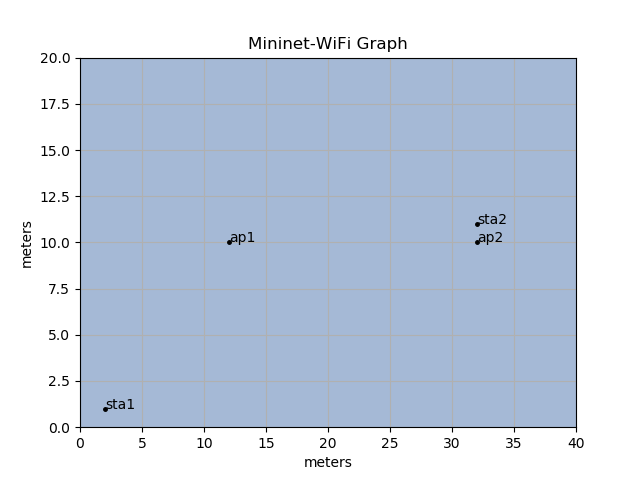
\includegraphics[scale=0.7]{Figuras/posicion.png}
		\caption{Posición de los nodos de la red meshAP.}
		\label{fig:pos}
	\end{figure}

Con la información que se tiene hasta el momento (la que aporta el script meshAP.py y la posición de los equipos de la red), se puede determinar que la topología de la red mesh es la indicada en la Figura \ref{fig:topo_inicial}, a falta de conocer cuáles son las interfaces que se conectan entre los diferentes equipos.\par

	\begin{figure}[!h]
		\centering
		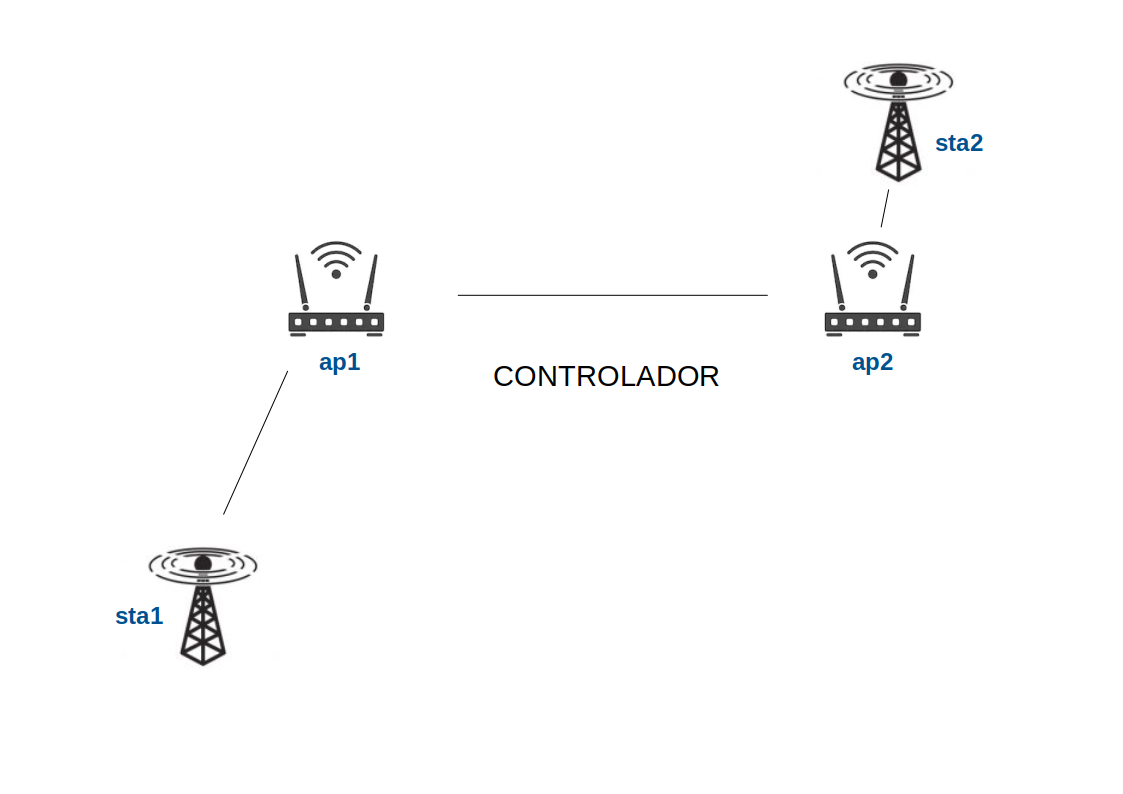
\includegraphics[scale=.4]{Figuras/topo_inicial.png}
		\caption{Topología de la red meshAP.}
		\label{fig:topo_inicial}
	\end{figure}

Sin embargo, aún falta conocer cuáles son las interfaces de los nodos, cómo se conectan entre ellas y qué papel tiene en estas conexiones el controlador de la red. En los siguientes apartados del presente capítulo se analizará el funcionamiento de la red en ejecución para comprender cómo funciona realmente una red mesh definida por software y poder completar el esquema de la topología de la red analizada.\par

\section{Establecimiento de la conexión y configuración de las interfaces}

\section{Análisis de los flujos de datos con \textit{pingall}}

\section{Topología completa resultante}



\end{document}